\documentclass{article}
\usepackage[polish]{babel}
\usepackage{amssymb}
\usepackage{graphicx}
\title{Sprawozdanie z Laboratorium 1}
\author{
  Hubert Rotkiewicz 193421 \and 
Dodaj siebie
}
\begin{document}
Miejsce na protokół
\maketitle
\section{Zadanie Z2}
\subsection{Opis Zadania}
\centering
Zadanie zostało wykonane z życiem oscyloskopu z laboratorium, Do kanału 1 podłączono diodę badaną,
kanał 2 podłączono do rezystora R2 o oporze 1 $\Omega$. 
\raggedright
\subsection{Wyniki}
\subsubsection{Dioda 1N4004}
\centering
\begin{figure}[h]
\centering
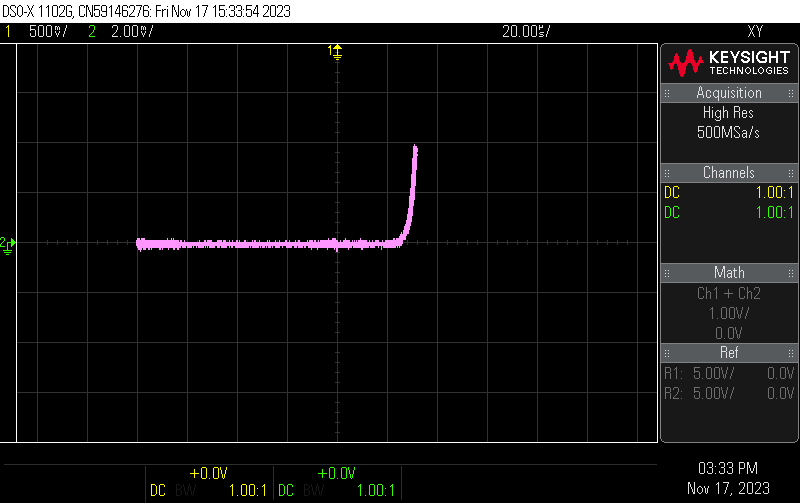
\includegraphics[scale=0.35]{./img/scope_0.png}
  \caption{Dane otrzymane z oscyloskopu dla diody 1N4004}
\end{figure}
Napięcie na kanale 2, jest równe wartości prądu płynącego przez diodę, ponieważ rezystor R2 ma opór 1 $\Omega$.
W notcie katalogowej producent podaje wartość "Forward Voltage" dla prądu 1A, wynosi 1 V. Z wykresu widać, że napięcie 
przewodzenia diody jest nieco mniejsze $\approx$ 0,8 V. Spowodowane jest to tym, że prąd płynący przez diodę jest mniejszy niż 1A. Można założyć, że napięcie przewodzenia zgadza się z tym podanym przez producenta.
\raggedright
\subsubsection{Dioda BAVP17}
\section{Zadanie Z3}
\centering
\subsection{Opis Zadania} 
Zmierzone zostały charakterystyka prądowo napięciowe z użyciem oscyloskopu metodą punkt po punkcie. 
Diodą badaną jest dioda czerwona LED. Wyniki pomiarów widoczne są w tabeli Z3 na protokole.
\begin{figure}[h]
\centering
  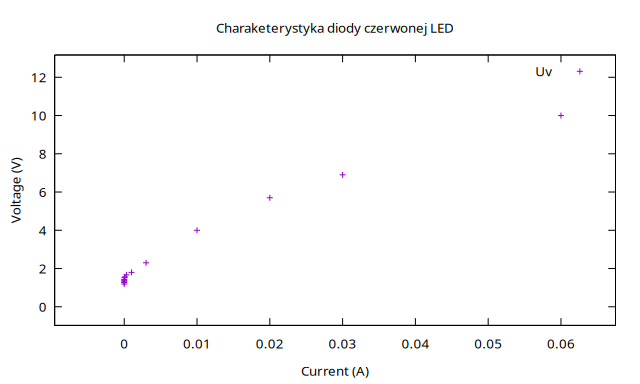
\includegraphics[scale=0.5]{./img/Z3_Uv.png}
  \caption{Napięcie zmierzone przez multimetr}
\end{figure}
Miejsce na Wykres Ua i U 


